% !TEX encoding = UTF-8 Unicode
% 予備審査レジュメ 案A(空間熱干渉の筋)で作り直した版・3 ページ(11/25、Claude 下書き → レオが読んで直す)。前の版は resume.tex(4 ページ)・resume2.tex(2 ページ)
% 図をページ幅で入れるため multicols ではなく twocolumn にした(11/22)
% ヘッダーは先輩(2025年度 7307)の「創造工学専攻 情報工学コース / 年度 特別研究 2 審査会」に合わせた
% ビルド:thesis/resume/ で latexmk resume.tex → build/resume.pdf
\documentclass[10pt,uplatex,dvipdfmx,twocolumn]{jsarticle}

% 描画・色関連
\usepackage[dvipdfmx]{graphicx}
\usepackage[dvipdfmx]{xcolor}
\usepackage{here}

% レイアウト調整関連
\usepackage{geometry}
\usepackage{setspace}
\usepackage{fancyhdr}
\usepackage{float}

% 数式関連
\usepackage{amsmath}
\usepackage{amssymb}
\usepackage{mathtools}
\usepackage{bm}

% 表・リスト関連
\usepackage{booktabs}
\usepackage{enumerate}

% テキスト装飾関連
\usepackage{url}

% キャプション関連
\usepackage{caption}
\usepackage{subcaption}

\graphicspath{{figures/}{../figures/}{../../experiments/}}
\geometry{a4paper, left=20mm,right=20mm,top=20mm,bottom=20mm}

\definecolor{tmcitblue}{cmyk}{0.86,0.91,0,0.04}
\pagestyle{fancy}
\fancyhf{}
\lhead{\color{tmcitblue}\footnotesize 東京都立産業技術高等専門学校}
\rhead{\color{tmcitblue}\footnotesize 専攻科 情報工学コース\\2026 年度特別研究Ⅱ予備審査会}
\lfoot{\color{tmcitblue}\footnotesize Tokyo Metropolitan College of Industrial Technology}
\cfoot{\thepage}
\renewcommand{\headrulewidth}{0.0pt}
\setlength{\headheight}{20.2781pt}
% ページ幅の図(figure*)をページの上に2つまで置けるように
\setcounter{dbltopnumber}{3}
\renewcommand{\dbltopfraction}{0.85}
\renewcommand{\dblfloatpagefraction}{0.85}
\renewcommand{\textfraction}{0.1}

% 節と図の前後の空きを詰める
\setlength{\textfloatsep}{8pt plus 2pt minus 2pt}
\setlength{\dbltextfloatsep}{8pt plus 2pt minus 2pt}
\captionsetup{skip=4pt}
\makeatletter
\renewcommand{\section}{\@startsection{section}{1}{\z@}{0.6\Cvs \@plus.3\Cdp}{0.3\Cvs}{\normalfont\large\headfont\raggedright}}
\renewcommand{\subsection}{\@startsection{subsection}{2}{\z@}{0.3\Cvs \@plus.2\Cdp}{0.1\Cvs}{\normalfont\normalsize\headfont}}
\makeatother

\begin{document}
\setstretch{1.00}
\twocolumn[{%
\centering
\Large{エッジマイクロクラスタにおける空間熱干渉を考慮した熱抑制手法の研究}\\
\vspace{6pt}
\large{7303 鈴木黎映}\\
\large{指導教員 知念賢一教授}
\vspace{10pt}
}]
% 赤字【】は結果待ち・要確認
\newcommand{\TBD}[1]{\textcolor{red}{【#1】}}

\section{はじめに}
データセンタでは、サーバの排熱が別のサーバの吸気側に回り込む熱の再循環が、冷却の効率を下げることが知られている~\cite{moore,tang}。同じことは、Raspberry Pi などの小型の計算機を棚や箱に密に並べたエッジのマイクロクラスタ~\cite{iridis}でも起こりうる。あるノードの排熱で隣のノードの温度が上がる現象を、本研究では空間熱干渉と呼ぶ。エッジの機器は空調のない場所に置かれることが多く、Raspberry Pi 4B(以下、Raspi)は CPU 温度が約 80\,℃ を超えるとクロックを下げて(スロットリング)処理が遅くなる。ファンを常に回せば温度は下がるが、ファンの寿命は稼働時間で表されるため~\cite{kim}、回し続けるほど寿命に近づき、騒音にもなる。そのため、スロットリングを避けつつ、ファンの稼働をできるだけ減らしたい。

先行発表~\cite{ipsj}では、空間熱干渉を外部熱影響 $H$ という状態として推定するカルマンフィルタを提案した。そこでは、密閉した容器に Raspi を並べると、隣のノードの負荷だけでアイドルのノードが約 12\,℃ 上がった。一方、本研究の予備的な測定では、開いたラックや机の上に横に並べた場合、隣のノードの上昇は 0.5\,℃ 未満であった。空間熱干渉が起こるかどうかは配置によって大きく変わるが、どのような配置で起こるのかは、これまで測られていなかった。

本研究では、まず、空間熱干渉がどの条件で起こるかを、ノードの位置関係(上下・左右・斜め)、発熱量、囲いの有無を変えて実機で測る。次に、空間熱干渉を推定に取り込んだ予測とファン制御が、干渉の起こる条件と起こらない条件でどう働くかを評価する。

\section{関連研究}
データセンタでは、熱の再循環を考慮した負荷の配置~\cite{moore,tang}が研究されている。計算機の内部では、熱 RC モデルによるモデル予測制御~\cite{zanini}や、温度を予測して先回りする熱管理~\cite{coskun,yeo}、予測のマージンを変動に応じて変える方法~\cite{sakamoto}がある。これらは部屋全体か 1 台の内部を対象としており、小型の計算機を密に並べたときにノードの間でどの程度熱が伝わるかを実測したものではない。

\section{提案手法}
\begin{figure*}[tb]
  \centering
  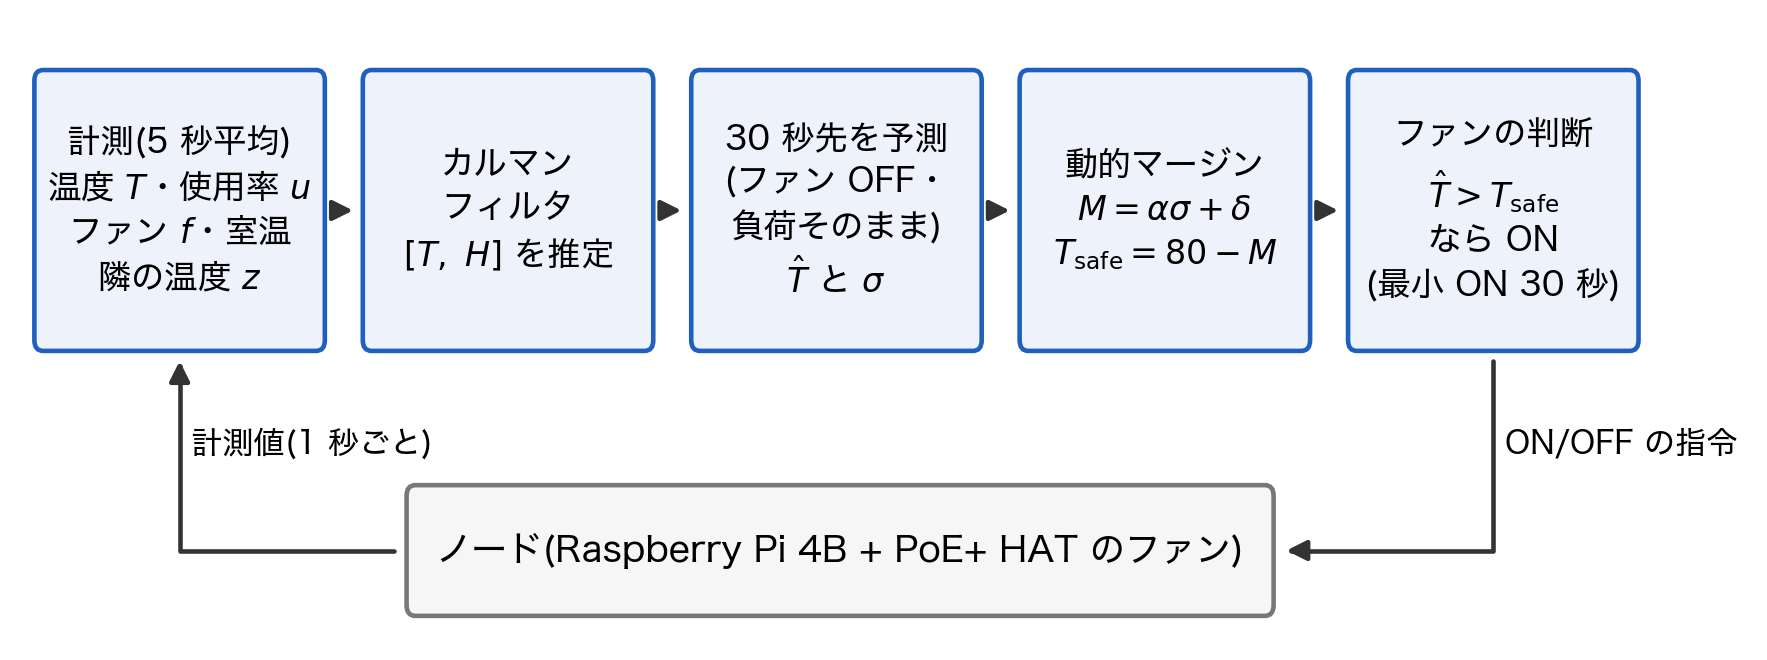
\includegraphics[width=0.68\textwidth]{fig_method_flow.png}
  \caption{提案手法の流れ(5 秒ごと)}
  \label{fig:flow}
\end{figure*}
手法の流れを図~\ref{fig:flow}に示す。5 秒ごとに、各ノードの温度・CPU 使用率・ファンの状態と隣接ノードの温度を観測し、30 秒先の温度とその不確かさを予測して、ファンを回すかどうかを決める。

\subsection{外部熱影響を含む熱モデル}
1 台のノードを熱 RC モデルで表して 5 秒ごとに離散化し、温度を室温からの上昇分 $\theta_t = T_t - T_{\mathrm{amb}}$ で表す。
\begin{gather}
  \theta_{t+1} = a\,\theta_t + b\,u_t + c\,H_t + e\,f_t + d + w^{\theta}_t \label{eq:theta}\\
  H_{t+1} = \rho\,H_t + (1-\rho)\,z_t + w^{H}_t \label{eq:h}
\end{gather}
$u_t$ は CPU 使用率、$f_t$ はファンの状態(0/1)である。$a$ は熱の残り方、$b > 0$ は負荷による加熱、$e < 0$ はファンによる冷却、$d$ は待機時の発熱を表す。$H_t$ が外部熱影響で、$z_t$ は隣接ノードの温度の、アイドル時の平均からの変化分である。隣が熱くなると $H_t$ がそれを $\rho$ でならしながら追いかけ、その影響が $c$ を通して自ノードに現れる。隣が熱くなって自ノードが冷えることはないため、$c \ge 0$ とする。空間熱干渉が起こらない配置では同定すると $c \approx 0$ となり、自ノードの負荷とファンだけのモデルに戻る。つまり、干渉の有無を前もって知らなくても、同じ手法を使える。

\subsection{推定・予測と動的マージン}
観測できるのは $\theta_t$ だけであり、カルマンフィルタで $\theta_t$ と $H_t$ を同時に推定する。隣接ノードの温度が急に変わったときは、$H$ のプロセスノイズを $q_H(t) = q_{H0} + \beta\,|z_t - z_{t-1}|$ と大きくする。推定した状態から 30 秒先の温度と誤差共分散 $P_{t+6|t}$ を求める。未来の負荷は分からないため今の負荷が続くと仮定し、「この先 30 秒回さなくても安全か」を判断するため、ファンは OFF のままと仮定する。30 秒は、ファンが効き始めるまでの時間(5 秒以内)より長く、温度の時定数(約 1〜2 分)より短い長さとした。
\begin{equation}
  M_t = \alpha\,\sigma_t + \delta,\qquad T_{\mathrm{safe}} = T_{\mathrm{limit}} - M_t
\end{equation}
$\sigma_t = \sqrt{P_{t+6|t}[0,0]}$、$\alpha = 2$、$\delta = 0.5$\,℃(温度センサの刻み)、$T_{\mathrm{limit}} = 80$\,℃ とした。隣の温度が急に変わり $c > 0$ であれば、$\sigma$ が広がってマージンが大きくなる。予測温度が $T_{\mathrm{safe}}$ を超えたらファンを ON にし、最小 ON 時間(30 秒)が過ぎて予測が $T_{\mathrm{safe}} - 1$\,℃ を下回ったら OFF にする。

\section{実験}
\subsection{何を確かめるか}
\begin{enumerate}
  \setlength{\itemsep}{0pt}\setlength{\parskip}{0pt}
  \item[Q1] 空間熱干渉は、どの位置関係(上・横・斜め・離れた位置)、どの発熱量、囲いの有無で起こるか
  \item[Q2] 冷やすときにも干渉は影響するか。(a) ファンの風で排熱が隣に運ばれるか。(b) 隣が熱いと自ノードのファンの冷え方が弱くなるか
  \item[Q3] 干渉が起こる条件で、$H$ を持つ予測は持たない予測より当たるか
  \item[Q4] 予測に基づくファン制御は、スロットリングを避けつつファンの稼働を減らせるか
\end{enumerate}
Q1〜Q3 の条件と判定の基準は、測定の前に決めて記録した。

\subsection{実験環境と条件}
\begin{figure}[tb]
  \centering
  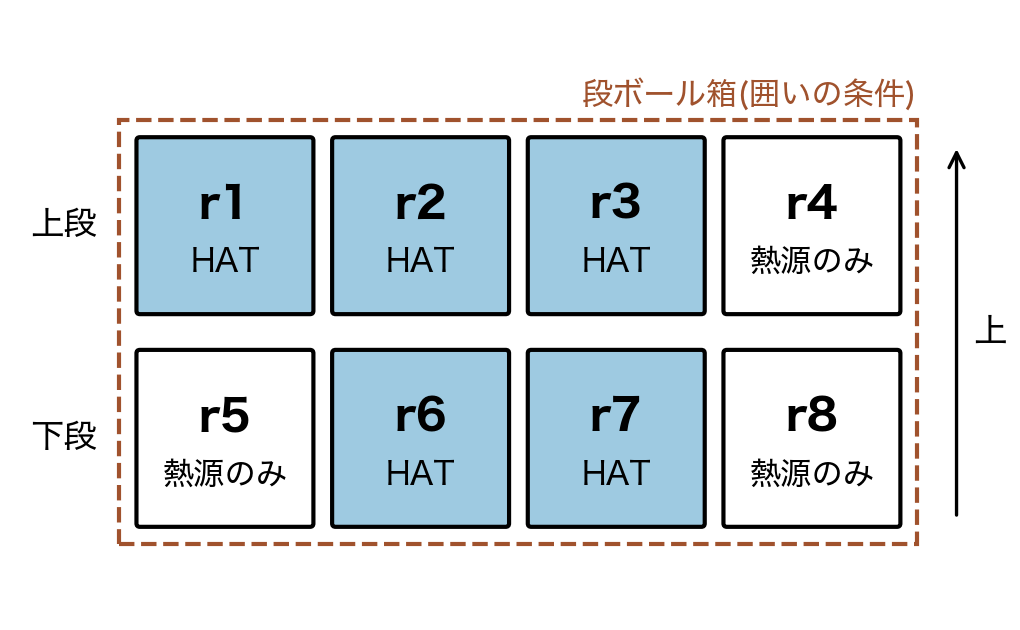
\includegraphics[width=0.9\columnwidth]{fig_rack_layout.png}
  \caption{ラックの配置(ポート側から見た図)。網掛けは PoE+ HAT(ファン付き)のあるノード}
  \label{fig:layout}
\end{figure}
Raspi 8 台(r1〜r8、Ubuntu 24.04)を 2 段 × 4 列のラックに縦向きに固定した(図~\ref{fig:layout})。5 台には PoE+ HAT を付けてファンを制御用 PC から ON/OFF し、残りの 3 台(PoE+ HAT が 5 個しかなかったため)はファンのない熱源として負荷だけを与えた。温度・CPU 使用率・クロック・スロットリングの状態・ファンの状態を 8 台すべてで 1 秒ごとに集め、部屋とラック(箱)の上部・正面の気温も記録した。PoE の給電電流から求めた 1 台の消費電力は、アイドルで約 2.4\,W、2 コアの負荷で約 3.8\,W であった\TBD{1 台だけ低く出る、要確認}。

囲いは、なし(ラックがむき出し)と、段ボール箱(307 × 220 × 120\,mm、約 8\,L)をラック全体にかぶせた状態(上・左右・後ろを覆い、正面と下は開いている。正面も閉じるとアイドルだけで箱の上部が 18 分で 39\,℃ まで上がり続けたため止めた)の 2 通りとした。それぞれで、2 コアの負荷 10 分と休み 12 分を 1 ブロックとして、r6 だけ・r7 だけ(位置関係)、下段 4 台・8 台すべて(発熱量)に負荷をかけた。Q2 (a) では r6 のファンを ON にしたまま r6 に負荷をかけ、(b) では r2 に負荷をかけて 10 分後に r2 のファンを ON にし、ほかの 7 台がアイドルのときと負荷のときを比べた。上昇は、負荷の最後 60 秒と直前 60 秒の平均温度の差から室温の変化を引いた値とし、1\,℃ 以上なら「干渉あり」とした。Q3 では、後半(全台に負荷がかかる)で同定し、前半(自ノードは休み、隣だけに負荷)のファン OFF の区間で、自ノードだけのモデル、$H$ を持つモデル(室温はどちらも部屋)、室温として上部または正面の気温を使う自ノードだけのモデルの 30 秒先の予測を比べた。Q4 は、横に 3 台並べた予備実験で、0〜4 コアの負荷を切り替える 20 分のパターンを 5 条件で 3 巡行って評価した。

\section{結果}
\begin{table}[tb]
  \centering
  \caption{負荷をかけていないノードの上昇(℃、室温の変化を引いた値)}
  \label{tab:pattern}
  \footnotesize\setlength{\tabcolsep}{2pt}
  \begin{tabular}{@{}lrr@{}}
    \toprule
    負荷 → 見るノード & 開いた状態 & 箱 \\
    \midrule
    真上(r6→r2, r7→r3) & $+0.1$, $+2.0$ & $-0.5$, $+0.5$ \\
    横(r6→r7, r7→r6) & $-1.4$, $+1.3$ & $-0.2$, $-0.2$ \\
    斜め上(r6→r1・r3, r7→r2) & $-0.3$, $-1.5$, $+1.0$ & $-0.1$, $-0.4$, $0.0$ \\
    離れた位置(r7→r1) & $+0.4$ & $+0.1$ \\
    下段 4 台 → 上段 r1〜r4 & $+0.6$〜$+1.4$ & $+0.1$〜$+1.8$ \\
    \bottomrule
  \end{tabular}
\end{table}
\subsection{空間熱干渉が起こる条件(Q1)}
結果を表~\ref{tab:pattern}に示す。開いた状態では $-1.5$〜$+2.0$\,℃ の範囲で、1\,℃ を超えたものもあるが逆向きではそろわず、部屋の温度の変化(3 時間で 2.8\,℃)によるブロックごとの揺れ(約 $\pm 1.5$\,℃)に埋もれた。箱では揺れが小さく、どの位置関係でも $\pm 0.5$\,℃ 以内であった。下段 4 台に負荷をかけると、上段の端の r1・r4 が $+1.8$・$+1.3$\,℃ 上がり、真上の r2・r3 は $+0.2$\,℃ 以下であった。

一方、囲うこと自体の影響は大きく、負荷の前の温度は部屋の温度の差を引いても開いた状態より 5〜10\,℃ 高かった。8 台に同時に負荷をかけると、箱ではファン付きの 5 台がすべて 83\,℃ に達して強制 ON とクロック低下が起き、開いた状態でも 4 台が 80〜83\,℃ に達した。

\subsection{冷やすときの干渉(Q2)と予測の精度(Q3)}
(a) r6 のファンを ON にしても、隣の上昇の差は揺れの範囲であった(箱では $\pm 0.4$\,℃ 以内)。(b) ファンを ON にすると、ほかの 7 台が休みでも負荷中でも r2 は同じだけ(開いた状態で 18.8\,℃、箱で 17〜18\,℃)下がった。開いた状態では隣も負荷のとき ON の時点で 3\,℃ 高く、その差が残った。

Q3:上段 r1〜r3 の 30 秒先の平均絶対誤差は、開いた状態で自ノードだけ 0.64、$H$ あり 0.39、上部・正面の気温を使う自ノードだけ 0.69・0.71\,℃、箱で 0.84、0.44、0.53・0.41\,℃ であった。$H$ は誤差を 0.25〜0.40\,℃ 小さくしたが、箱では正面の気温を使うモデルと同じ精度であった。

\subsection{ファン制御(Q4)}
\begin{table}[tb]
  \centering
  \caption{ファン制御の結果(予備実験、9 回の平均)}
  \label{tab:control}
  \small
  \begin{tabular}{lrrr}
    \toprule
    条件 & 稼働率 & 最高温度 & 80\,℃ 超過 \\
    \midrule
    ファンなし & 14\%$^{*}$ & 83.6\,℃ & 696 秒 \\
    常時 ON & 100\% & 65.0\,℃ & 0 \\
    しきい値(75/70\,℃) & 40\% & 78.4\,℃ & 0 \\
    予測 + 固定マージン & 45\% & 76.8\,℃ & 0 \\
    提案 & 38\% & 78.7\,℃ & 0 \\
    \bottomrule
    \multicolumn{4}{l}{\footnotesize $^{*}$ 82\,℃ 以上での安全のための強制 ON の分}
  \end{tabular}
\end{table}
表~\ref{tab:control}に示すように、予測を用いる 2 方式としきい値方式は、すべての回で 80\,℃ を超えなかった。提案手法は常時 ON と比べてファンの稼働を約 6 割減らし、干渉のない配置で $c \approx 0$ となっても壊れずに働いた。一方、しきい値方式との差はほぼなかった。

\section{考察}
\subsection{空間熱干渉が起こる条件と $H$ の役割}
空間熱干渉を「ほかのノードの発熱によって自ノードの温度が上がること」とし、熱の経路は問わない。1 台の排気が隣を直接温める経路は、位置関係によらず 1\,℃ 未満であった。一方、囲いやラックの空気に熱が溜まる経路は大きく、考慮が要るのは囲いの閉じ方と同時に動く台数である。先行発表の約 12\,℃ の上昇も、密閉した小さな容器で溜まる経路が効いた結果と考えられる。

箱では箱の中の気温を使うモデルが $H$ と同じくらい当たり、測定前に決めた解釈では、箱の中の干渉は主に箱全体の昇温で、$H$ の役割は「箱の中に温度計がないときに、隣の温度からその昇温を推定する」ことである。開いた状態では、どの気温を使っても $H$ ほど当たらなかった。

\subsection{しきい値方式と差がなかった理由}
PoE+ HAT のファンは 5 秒以内に効き始め効果も大きいため、温度が上がってから回しても間に合い、予測の利点が小さい。シミュレーションでは、効き始めが 15〜30 秒以上遅れると予測を用いる方式が少ない稼働で 80\,℃ を守った。Q2 (b) では隣が熱くてもファンの効きは弱まらず、干渉は温度の水準を押し上げるだけであった。予測が役立つのは、より遅い冷却の場合と考えられる。

\section{おわりに}
Raspi 8 台のラックで、位置関係・発熱量・囲い・ファンを変えて、空間熱干渉が起こる条件を実測した。1 台の排気が隣を直接温める干渉は 1\,℃ 未満で、熱は囲いやラックの空気に溜まる形で効いていた。$H$ は 30 秒先の予測誤差を 0.25〜0.40\,℃ 小さくし、箱の中の気温を使うのと同じ精度であった。今後は囲いの大きさ・閉じ方と発熱量を変えて溜まる経路が効き始める条件を調べ、干渉が起こる配置でファン制御を評価する。

\scriptsize{
\begin{thebibliography}{99}
  \setlength{\itemsep}{0pt}
  \bibitem{moore} J. Moore et al., ``Making Scheduling ``Cool'': Temperature-Aware Workload Placement in Data Centers,'' USENIX ATC, pp.61--74, 2005.
  \bibitem{tang} Q. Tang et al., ``Energy-Efficient Thermal-Aware Task Scheduling for Homogeneous HPC Data Centers,'' IEEE TPDS, Vol.19, No.11, pp.1458--1472, 2008.
  \bibitem{iridis} S. J. Cox et al., ``Iridis-pi: a low-cost, compact demonstration cluster,'' Cluster Computing, pp.349--358, 2014.
  \bibitem{kim} S. J. Kim, A. Claassen, ``How to Evaluate Fan Life,'' Electronics Cooling, 1996.
  \bibitem{ipsj} 鈴木 黎映, 知念 賢一, ``空間熱干渉を考慮した状態推定に基づく動的熱マージン制御手法,'' 情報処理学会研究報告, Vol.2026-OS-171, No.3, 2026.
  \bibitem{zanini} F. Zanini et al., ``Multicore Thermal Management with Model Predictive Control,'' Proc. ECCTD, pp.711--714, 2009.
  \bibitem{sakamoto} 坂本 竜 他, ``仮想マシンの CPU 使用率の負荷予測に対する安定度を用いた動的マージン設定手法,'' 信学技報, Vol.117, No.465, pp.49--54, 2018.
  \bibitem{coskun} A. K. Coskun et al., ``Proactive Temperature Management in MPSoCs,'' Proc. ISLPED, 2008.
  \bibitem{yeo} I. Yeo et al., ``Predictive Dynamic Thermal Management for Multicore Systems,'' Proc. DAC, pp.734--739, 2008.
\end{thebibliography}
}
\end{document}
